\documentclass{beamer}
% Use DS9 global theme
\usepackage{../../../shared/templates/ds9_theme}

% Title page configuration
\title[Unit 1 Review]{PHYS12 CH123:}
\subtitle{Test Prep}
\author[Mr. Gullo]{Mr. Gullo}
\date[Oct 2024]{October 2024}


\begin{document}

\frame{\titlepage}

\section{Introduction}

\begin{frame}
\frametitle{Overview}
\begin{itemize}
    \item Review of key concepts from Chapters 1-3
    \item Practice problems with step-by-step solutions
    \item Focus on:
    \begin{itemize}
        \item Significant figures and uncertainties
        \item Unit conversions
        \item Velocity and displacement calculations
        \item Vector addition
    \end{itemize}
\end{itemize}
\end{frame}

\section{Chapter 1: Measurement and Problem Solving}
\begin{frame}
\frametitle{Problem 1: Significant Figures and Uncertainties}
\begin{block}{Question}
(a) How many significant figures are in the numbers 99 and 100?\\
(b) If the uncertainty in each number is 1, what is the percent uncertainty in each?\\
(c) Which is a more meaningful way to express the accuracy of these two numbers, significant figures or percent uncertainties?
\end{block}
\end{frame}

\begin{frame}
\frametitle{Problem 1: Solution (Part a)}
\begin{block}{Question}
(a) How many significant figures are in the numbers 99 and 100?\\
\end{block}
\begin{block}{Solution}
(a) 99 has \underline{2} sig. figs.; 100 has \underline{3} sig. figs. at most
\end{block}
\begin{block}{Explanation}
\begin{itemize}
\item For 99: Both digits are non-zero, so both are significant.
\item For 100: The 1 is non-zero, so it's significant. The zeros to the right of a non-zero digit are potentially significant. If this is an exact number, it has 1 sig. fig. If it's a measurement, it could have up to 3 sig. figs.
\item Always clarify with the context whether trailing zeros are significant.
\end{itemize}
\end{block}
\end{frame}
\begin{frame}
\frametitle{Significant Figures in 100}

\begin{columns}[T]
\column{0.33\textwidth}
\begin{exampleblock}{3 Significant Figures}
\textbf{Example:} Digital scale reads 100 g
\begin{itemize}
\item All digits significant
\item Precise to nearest gram
\item Written as 1.00 × 10² g
\end{itemize}
\end{exampleblock}

\column{0.33\textwidth}
\begin{exampleblock}{1 Significant Figure}
\textbf{Example:} About 100 people
\begin{itemize}
\item Only 1 is significant
\item Estimate or rounding
\item Written as 1 × 10² people
\end{itemize}
\end{exampleblock}

\column{0.33\textwidth}
\begin{exampleblock}{Infinite Significant Figures}
\textbf{Example:} Exact numbers
\begin{itemize}
\item 100 cents in a dollar
\item 100 years in a century
\item Defined, not measured
\end{itemize}
\end{exampleblock}
\end{columns}
\end{frame}


\begin{frame}
\frametitle{Problem 1: Solution (Part b)}
\begin{block}{Question}
(b) If the uncertainty in each number is 1, what is the percent uncertainty in each?\\
\end{block}
\begin{block}{Solution}
(b) For 99: $\frac{1}{99} \times 100 = 1.01\% = \underline{1.0\%}$\\
   For 100: $\frac{1}{100} \times 100 = \underline{1.00\%}$ (if all zeros are significant)
\end{block}
\begin{block}{Explanation}
\begin{itemize}
\item Percent uncertainty = $\frac{\text{absolute uncertainty}}{\text{measured value}} \times 100\%$
\item For 99: $\frac{1}{99} \times 100 = 1.01\%$, rounded to 1.0\% (2 sig. figs.)
\item For 100: $\frac{1}{100} \times 100 = 1.00\%$ (3 sig. figs. if all zeros are significant)
\item Note: The uncertainty in the result should not be more precise than the given uncertainty (1).
\end{itemize}
\end{block}
\end{frame}

\begin{frame}
\frametitle{Problem 1: Solution (Part c)}
\begin{block}{Question}
(c) Which is a more meaningful way to express the accuracy of these two numbers, significant figures or percent uncertainties?
\end{block}
\begin{block}{Solution}
(c) Percent uncertainties are a more meaningful way to express the accuracy of these two numbers.
\end{block}
\begin{block}{Explanation}
\begin{itemize}
\item Significant figures give a rough idea of precision, but can be ambiguous (e.g., for 100).
\item Percent uncertainty provides a clear, quantitative measure of relative accuracy.
\item In this case, percent uncertainty shows that both numbers have similar accuracy (about 1\%), which isn't clear from sig. figs. alone.
\item Percent uncertainty is particularly useful for comparing measurements with different magnitudes.
\end{itemize}
\end{block}
\end{frame}\begin{frame}
\frametitle{Problem 1: Solution (Part c)}
\begin{block}{Solution}
(c) Percent uncertainties are a more meaningful way to express the accuracy of these two numbers.
\end{block}
\begin{block}{Explanation}
\begin{itemize}
\item Significant figures give a rough idea of precision, but can be ambiguous (e.g., for 100).
\item Percent uncertainty provides a clear, quantitative measure of relative accuracy.
\item In this case, percent uncertainty shows that both numbers have similar accuracy (about 1\%), which isn't clear from sig. figs. alone.
\item Percent uncertainty is particularly useful for comparing measurements with different magnitudes.
\end{itemize}
\end{block}
\end{frame}
\begin{frame}
\frametitle{Problem 2: Percent Uncertainty}
\begin{block}{Question}
(a) A person's blood pressure is measured to be $120 \pm 2$ mm Hg. What is its percent uncertainty?\\
(b) Assuming the same percent uncertainty, what is the uncertainty in a blood pressure measurement of 80 mm Hg?
\end{block}
\end{frame}

\begin{frame}
\frametitle{Problem 2: Solution (Part a)}
\begin{block}{Solution}
(a) $\% unc = \frac{2 \text{ mm Hg}}{120 \text{ mm Hg}} \times 100\% = 1.7\% = \underline{2\%}$\\
(1 sig. fig because of 2 mm Hg)
\end{block}
\end{frame}

\begin{frame}
\frametitle{Problem 2: Solution (Part b)}
\begin{block}{Solution}
(b) $\delta bp = \frac{1.7\%}{100\%} \times 80 \text{ mm Hg} = 1.3 \text{ mm Hg} = \underline{1 \text{ mm Hg}}$\\
(1 sig. fig because of 2 mm Hg)
\end{block}
\end{frame}

\begin{frame}
\frametitle{Problem 3: Uncertainty and Unit Conversion}
\begin{block}{Question}
(a) A car speedometer has a 5.0\% uncertainty. What is the range of possible speeds when it reads 90 km/h?\\
(b) Convert this range to miles per hour. (1 km = 0.6214 mi)
\end{block}
\end{frame}

\begin{frame}
\frametitle{Problem 3: Solution (Part a)}
\begin{block}{Solution}
(a) $\delta v = \frac{5.0\%}{100\%} \times 90.0 \text{ km/h} = 4.5 \text{ km/h}$\\
Thus, the range = $90.0 \pm 5 \text{ km/h} = 85 \text{ to } 95 \text{ km/h}$.
\end{block}
\end{frame}

\begin{frame}
\frametitle{Problem 3: Solution (Part b)}
\begin{block}{Solution}
(b) Converting to miles per hour:
\begin{align*}
\frac{85.5 \text{ km}}{1 \text{ h}} \times \frac{0.6214 \text{ mi}}{1 \text{ km}} &= 53.1 \text{ mi/h}\\
\frac{94.5 \text{ km}}{1 \text{ h}} \times \frac{0.6214 \text{ mi}}{1 \text{ km}} &= 58.7 \text{ mi/h}
\end{align*}
So the range is 53.1 to 58.7 mi/h
\end{block}
\end{frame}

\section{Chapter 2 and 3: Motion in One and Two Dimensions}

\begin{frame}
\frametitle{Problem 4: Displacement and Time}
\begin{block}{Question}
Land west of the San Andreas fault in southern California is moving at an average velocity of about 6 cm/y northwest relative to land east of the fault. Los Angeles is west of the fault and may thus someday be at the same latitude as San Francisco, which is east of the fault. How far in the future will this occur if the displacement to be made is 590 km northwest, assuming the motion remains constant?
\end{block}
\end{frame}

\begin{frame}
\frametitle{Problem 4: Visualization}

\begin{tikzpicture}[scale=0.7]
    \draw[thick, ->] (0,0) -- (-10,0) node[left] {West};
    \draw[thick, ->] (0,0) -- (0,6) node[above] {North};
    
    % San Andreas Fault
    \draw[red, thick] (-1,-0.5) -- (-5,6.5);
    \node[red] at (-2.5,6) {San Andreas Fault};
    
    % Los Angeles
    \filldraw[blue] (-2,1) circle (2pt) node[below] {LA};
    
    % San Francisco
    \filldraw[green] (-6,5) circle (2pt) node[above] {SF};
    
    % Motion vector
    \draw[->, thick, orange] (-2,1) -- (-6,5);
    \node[orange] at (-5,3.5) {590 km};
    
    % Velocity vector
    \draw[->, thick, purple] (-2,1) -- (-2.3,1.3);
   \node[purple] at (-3.7,1.5) {6 cm/y};
    
    % Simple Compass Rose
    \draw[thick] (8,5) -- (8,6) node[above] {N};
    \draw[thick] (8,5) -- (7,5) node[left] {W};
    \draw[thick] (8,5) -- (9,5) node[right] {E};
    \draw[thick] (8,5) -- (8,4) node[below] {S};
\end{tikzpicture}
\end{frame}

\frametitle{Problem 4: Solution}
\begin{block}{Equations}
Velocity equation: $v = \frac{\Delta x}{\Delta t}$
Rearranged for time: $\Delta t = \frac{\Delta x}{v}$
\end{block}
\begin{block}{Solution}
\begin{align*}
\Delta t &= \frac{\Delta x}{v} = \frac{590 \text{ km}}{6 \text{ cm/year}} \times \frac{100000 \text{ cm}}{1 \text{ km}}\\
&= \frac{5.90 \times 10^5 \text{ m}}{6 \text{ cm/year}} \times \frac{100 \text{ cm}}{1 \text{ m}}\\
&= 9.83 \times 10^6 \text{ years} = 1 \times 10^7 \text{ years}\\
&= \underline{10 \text{ million years}}
\end{align*}
\end{block}
\end{frame}

\begin{frame}
\frametitle{Problem 5: Relative Motion (Part 1)}
\begin{block}{Question}
A seagull flies at a velocity of 9.00 m/s straight into the wind.
(a) If it takes the bird 20.0 min to travel 6.00 km relative to the Earth, what is the velocity of the wind?\\
(b) If the bird turns around and flies with the wind, how long will he take to return 6.00 km?\\
(c) Discuss how the wind affects the total round-trip time compared to what it would be with no wind.
\end{block}
\end{frame}

\begin{frame}
\frametitle{Problem 5: Visualization}
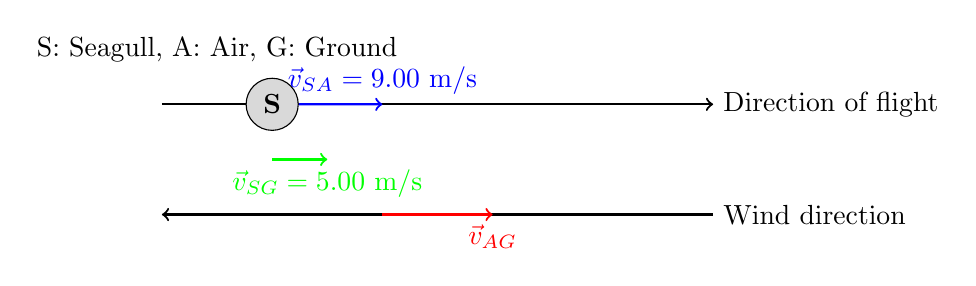
\begin{tikzpicture}[scale=0.7]
    \draw[thick, ->] (0,3) -- (10,3) node[right] {Direction of flight};
    \draw[thick, <-] (0,1) -- (10,1) node[right] {Wind direction};
    
    % Seagull
    \node[draw, circle, fill=gray!30] at (2,3) (seagull) {\textbf{S}};
    \draw[->, thick, blue] (seagull) -- ++(2,0) node[above] {$\vec{v}_{\text{SA}} = 9.00$ m/s};
    
    % Wind
    \draw[->, thick, red] (4,1) -- ++(2,0) node[below] {$\vec{v}_{\text{AG}}$};
    
    % Ground velocity
    \draw[->, thick, green] (2,2) -- ++(1,0) node[below] {$\vec{v}_{\text{SG}} = 5.00$ m/s};
    
    % Labels
    \node at (1,4) {S: Seagull, A: Air, G: Ground};
\end{tikzpicture}
\end{frame}

\begin{frame}
\frametitle{Problem 5: Solution (Part a)}
\begin{block}{Equations}
Relative velocity: $\mathbf{v}_{\mathbf{SG}} = \mathbf{v}_{\mathbf{SA}} + \mathbf{v}_{\mathbf{AG}}$
Rearranged for wind velocity: $\mathbf{v}_{\mathbf{AG}} = \mathbf{v}_{\mathbf{SG}} - \mathbf{v}_{\mathbf{SA}}$
Velocity from displacement and time: $v = \frac{x}{t}$
\end{block}
\begin{block}{Solution}
(a) Let A = air, S = seagull, G = ground
\begin{align*}
v_{\text{SG}} &= \frac{x_{\text{SG}}}{t} = \frac{6.00 \times 10^3 \text{ m}}{(20 \text{ min})(60 \text{ s/1 min})} = 5.00 \text{ m/s}\\
v_{AG} &= v_{\text{SG}} - v_{\text{SA}} = 5.00 \text{ m/s} - 9.00 \text{ m/s} = -4.00 \text{ m/s}
\end{align*}
\end{block}
\end{frame}

\begin{frame}
\frametitle{Problem 5: Solution (Part b)}
\begin{block}{Equations}
Relative velocity (with wind): $v_{\text{SG}} = v_{\text{SA}} - v_{\text{AG}}$
Time from displacement and velocity: $t = \frac{x}{v}$
\end{block}
\begin{block}{Solution}
(b) Flying with the wind:
\begin{align*}
v_{\text{SG}} &= v_{\text{SA}} - v_{\text{AG}} = 9.00 \text{ m/s} - (-4.00 \text{ m/s}) = 13.00 \text{ m/s}\\
t &= \frac{x_{\text{SG}}}{v_{\text{SG}}} = \frac{6.00 \times 10^3 \text{ m}}{13.00 \text{ m/s}} = 462 \text{ s} = \underline{7 \text{ min} \text{ 42 s}}
\end{align*}
\end{block}
\end{frame}

\begin{frame}
\frametitle{Problem 5: Solution (Part c)}
\begin{block}{Solution}
(c) The wind will always slow down the round trip time, relative to having no wind present.
\end{block}
\end{frame}

\begin{frame}
\frametitle{Problem 6: Vector Addition (Part 1)}
\begin{block}{Question}
A football quarterback is moving straight backward at a speed of 2.00 m/s when he throws a pass to a player 18.0 m straight downfield. The ball is thrown at an angle of 25.0° relative to the ground and is caught at the same height as it is released. \\What is the initial velocity of the ball relative to the quarterback?
\end{block}
\end{frame}

\begin{frame}
\frametitle{Problem 6: Visualization}
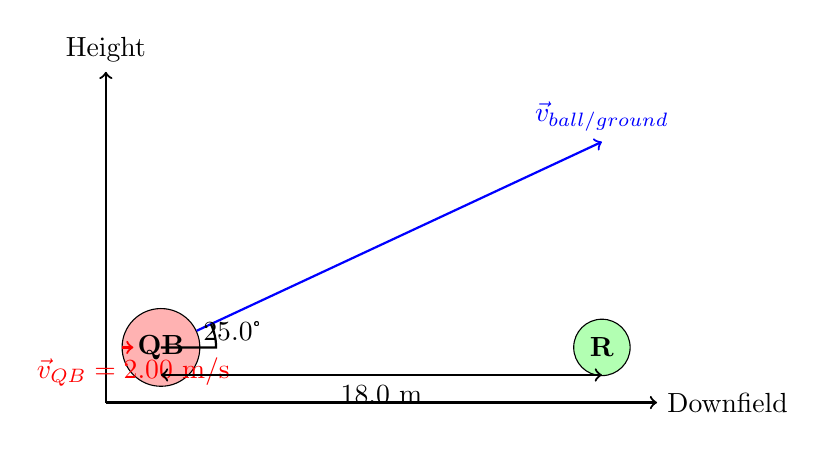
\begin{tikzpicture}[scale=0.7]
    \draw[thick, ->] (0,0) -- (10,0) node[right] {Downfield};
    \draw[thick, ->] (0,0) -- (0,6) node[above] {Height};
    
    % Quarterback
    \node[draw, circle, fill=red!30] at (1,1) (qb) {\textbf{QB}};
    \draw[->, thick, red] (qb) -- ++(-0.5,0) node[below] {$\vec{v}_{QB} = 2.00$ m/s};
    
    % Ball trajectory
    \draw[->, thick, blue] (qb) -- ++(8,3.73) node[above] {$\vec{v}_{ball/ground}$};
    
    % Angle
    \draw[thick] (1,1) -- ++(1,0) arc (0:25:1);
    \node at (2.3,1.3) {25.0°};
    
    % Receiver
    \node[draw, circle, fill=green!30] at (9,1) (receiver) {\textbf{R}};
    
    % Distance
    \draw[<->, thick] (1,0.5) -- (9,0.5) node[midway, below] {18.0 m};
\end{tikzpicture}
\end{frame}

\begin{frame}
\frametitle{Problem 6: Vector Addition Visualization}
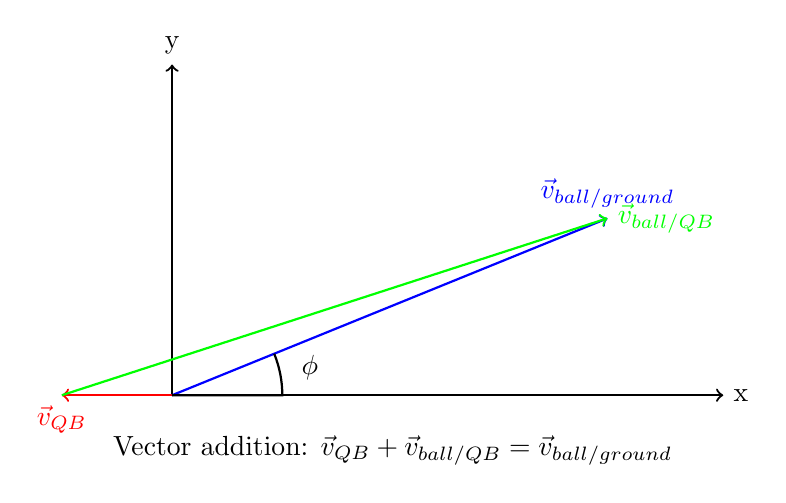
\begin{tikzpicture}[scale=0.7]
    \draw[thick, ->] (0,0) -- (10,0) node[right] {x};
    \draw[thick, ->] (0,0) -- (0,6) node[above] {y};
    
    % Quarterback's velocity vector
    \draw[->, thick, red] (0,0) -- (-2,0) node[below] {$\vec{v}_{QB}$};
    
    % Ball's velocity vector relative to ground
    \draw[->, thick, blue] (0,0) -- (7.9,3.21) node[above] {$\vec{v}_{ball/ground}$};
    
    % Ball's velocity vector relative to quarterback
    \draw[->, thick, green] (-2,0) -- (7.9,3.21) node[right] {$\vec{v}_{ball/QB}$};
    
    % Angle
    \draw[thick] (0,0) -- (2,0) arc (0:22.1:2);
    \node at (2.5,0.5) {$\phi$};
    
    % Labels
    \node at (4,-1) {Vector addition: $\vec{v}_{QB} + \vec{v}_{ball/QB} = \vec{v}_{ball/ground}$};
\end{tikzpicture}
\end{frame}

\begin{frame}
\frametitle{Problem 6: Solution (Part 1)}
\begin{block}{Equations}
Vector addition: $\vec{v}_{QB} + \vec{v}_{ball/QB} = \vec{v}_{ball/ground}$\\
Component equations:\\ 
$v_{QB_x} + v_{ball/QB_x} = v_{ball/ground_x} = v_{ball/ground} \cos \phi$\\
$v_{QB_y} + v_{ball/QB_y} = v_{ball/ground_y} = v_{ball/ground} \sin \phi$
\end{block}
\begin{block}{Solution}
(relative to ground)
\begin{align*}
v_{QB_x} + v_{ball/QB_x} &= v_{ball/ground} \cos \phi \\
-2 \text{ m/s} + v_{ball/QB_x} &= (15.2 \text{ m/s}) \cos 25.0° \Rightarrow v_{ball/QB_x} = 15.8 \text{ m/s}\\
v_{QB_y} + v_{ball/QB_y} &= v_{ball/ground} \sin \phi \\
0 + v_{ball/QB_y} &= (15.2 \text{ m/s}) \sin 25.0° \Rightarrow v_{ball/QB_y} = 6.42 \text{ m/s}
\end{align*}
\end{block}
\end{frame}

% Title page configuration
\title[Projectile Motion Analysis]{PHYS11 CH4:}
\subtitle{Projectile Motion Analysis: Quarterback Problem}
\author[Mr. Gullo]{Mr. Gullo}
\date[Oct 2024]{October 2024}


\begin{frame}
\frametitle{Quarterback Velocity Problem}
\begin{block}{Problem Context}
\begin{itemize}
    \item Quarterback moving backward at 2.00 m/s
    \item Ball thrown at 25.0° angle relative to ground
    \item Ball travels 18.0 m downfield
\end{itemize}
\end{block}

\begin{block}{Calculation Steps}
\begin{enumerate}
    \item Use projectile motion equation: $R = \frac{v^2 \sin(2\theta)}{g}$
    \item Rearrange to solve for v: $v = \sqrt{\frac{R g}{\sin(2\theta)}}$
    \item Given: $R = 18.0$ m, $\theta = 25.0°$, $g = 9.8$ m/s$^2$
    \item Calculate: $v \approx 15.2$ m/s
\end{enumerate}
\end{block}

\begin{alertblock}{Key Point}
The calculated velocity (15.2 m/s) is relative to the ground, not the quarterback.
\end{alertblock}
\end{frame}



\begin{frame}
\frametitle{Problem 6: Solution (Part 2)}
\begin{block}{Equations}
Magnitude of velocity vector: $v = \sqrt{v_x^2 + v_y^2}$
Angle of velocity vector: $\theta = \tan^{-1}\left(\frac{v_y}{v_x}\right)$
\end{block}
\begin{block}{Solution}
\begin{align*}
v_{ball/QB} &= \sqrt{v_{ball/QB_x}^2 + v_{ball/QB_y}^2} = \sqrt{(15.8 \text{ m/s})^2 + (6.42 \text{ m/s})^2} = \\\underline{17.0 \text{ m/s}}\\
\theta &= \tan^{-1}\left(\frac{v_{ball/QB_y}}{v_{ball/QB_x}}\right) = \tan^{-1}\left(\frac{6.42}{15.8}\right) = \underline{22.1°}
\end{align*}
\end{block}
\end{frame}

\begin{frame}
\frametitle{Problem 6: Vector Addition Visualization}
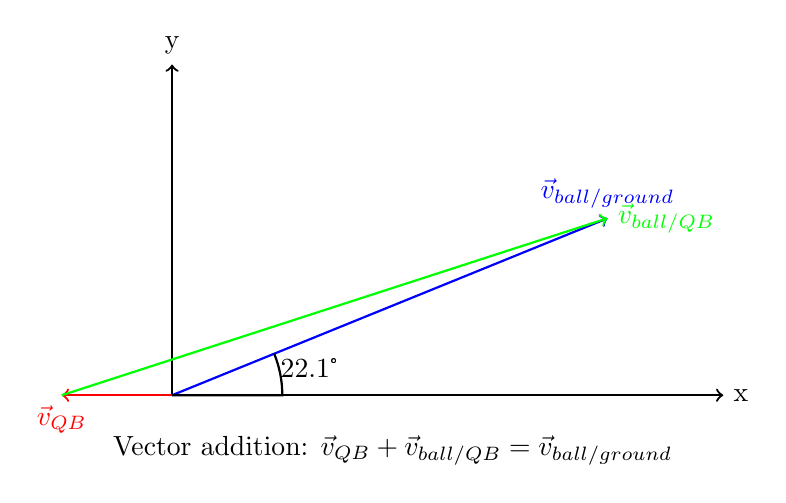
\begin{tikzpicture}[scale=0.7]
    \draw[thick, ->] (0,0) -- (10,0) node[right] {x};
    \draw[thick, ->] (0,0) -- (0,6) node[above] {y};
    
    % Quarterback's velocity vector
    \draw[->, thick, red] (0,0) -- (-2,0) node[below] {$\vec{v}_{QB}$};
    
    % Ball's velocity vector relative to ground
    \draw[->, thick, blue] (0,0) -- (7.9,3.21) node[above] {$\vec{v}_{ball/ground}$};
    
    % Ball's velocity vector relative to quarterback
    \draw[->, thick, green] (-2,0) -- (7.9,3.21) node[right] {$\vec{v}_{ball/QB}$};
    
    % Angle
    \draw[thick] (0,0) -- (2,0) arc (0:22.1:2);
    \node at (2.5,0.5) {22.1°};
    
    % Labels
    \node at (4,-1) {Vector addition: $\vec{v}_{QB} + \vec{v}_{ball/QB} = \vec{v}_{ball/ground}$};
\end{tikzpicture}
\end{frame}

\section{Conclusion}

\begin{frame}
\frametitle{Key Takeaways}
\begin{itemize}
    \item Importance of significant figures and uncertainties in measurements
    \item Proper use of unit conversions
    \item Understanding relative motion and vector addition
    \item Practice solving multi-step problems
    \item Always check units and reasonableness of answers
\end{itemize}
\end{frame}

\section{Problem 37: Tennis Serve}

\begin{frame}
\frametitle{Problem 37: Tennis Serve}
\begin{block}{Question}
A tennis player serves at a speed of $170 \mathrm{~km} / \mathrm{h}$ from a height of 2.5 m and an angle $\boldsymbol{\theta}$ below the horizontal. The baseline is 11.9 m from the net, which is 0.91 m high.\\
What is the angle $\theta$ such that the ball just crosses the net?\\
Will the ball land in the service box, which has an outermost service line 6.40 m from the net?
\end{block}
\end{frame}

\begin{frame}
\frametitle{Problem 37: Solution (Part 1)}
\begin{itemize}
    \item Convert initial velocity:
    $$v_{0}=170 \mathrm{~km} / \mathrm{h}=47.2 \mathrm{~m} / \mathrm{s}$$
    \item Calculate vertical distance to net:
    $$y=2.50 \mathrm{~m}-0.91 \mathrm{~m}=1.59 \mathrm{~m}$$
    \item Use kinematic equation:
    $$y=v_{0y} t+\frac{1}{2} a t^{2}$$
\end{itemize}
\end{frame}

\begin{frame}
\frametitle{Problem 37: Solution (Part 2)}
\begin{itemize}
    \item In x-direction:
    $$x=11.9 \mathrm{m}=(47.2 \mathrm{~m} / \mathrm{s})(\cos \theta) t$$
    $$t= \frac{0.252}{\cos \theta}$$
    \item Substitute into kinematic equation:
    $$1.59 \mathrm{~m}=(11.9 \mathrm{~m}) \tan \theta+(0.311 \mathrm{~m})(1+\tan ^{2} \theta)$$
    \item Solve for $\theta$:
    $$\tan \theta=0.107 \text{ or } \underline{\theta}=6.1^{\circ}$$
\end{itemize}
\end{frame}

\begin{frame}

\frametitle{Problem 37: Solution (Part 3)}
\begin{itemize}
    \item Calculate time for ball to fall 2.5 m:
    $$t=0.366 \mathrm{~s}$$
    \item Calculate range:
    $$R=v_{x} t= 17.2 \mathrm{~m}$$
    \item Answer: Yes, the ball lands 5.3 m from the net, within the service box.
\end{itemize}
\end{frame}

\section{Problem 39: Gun Sights}

\begin{frame}
\frametitle{Problem 39: Gun Sights}
\begin{block}{Question}
(a) A gun is sighted to hit targets at the same height, 100.0 m away. How low will the bullet hit if aimed at a target 150.0 m away? The muzzle velocity is $275 \mathrm{~m} / \mathrm{s}$.\\

(b) Discuss qualitatively how a larger muzzle velocity would affect this problem and what would be the effect of air resistance.
\end{block}

\end{frame}

\begin{frame}
\frametitle{Problem 39: Gun Sights}
\begin{block}{Question}
(a) A gun is sighted to hit targets at the same height, 100.0 m away. How low will the bullet hit if aimed at a target 150.0 m away? The muzzle velocity is $275 \mathrm{~m} / \mathrm{s}$.\\

(b) Discuss qualitatively how a larger muzzle velocity would affect this problem and what would be the effect of air resistance.
\end{block}
\begin{figure}[H]
    \centering
    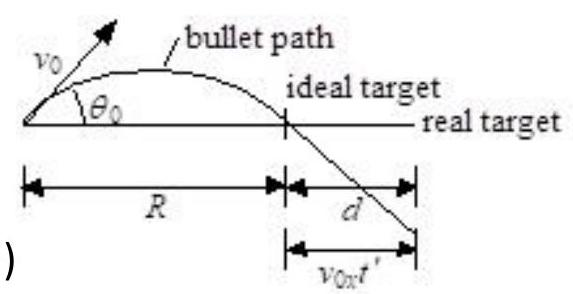
\includegraphics[width=0.75\linewidth]{CH123 Review/2024_09_22_a7542cd95c5ad1b43cb7g-23.jpg}
\end{figure}

\end{frame}

\begin{frame}
\frametitle{Problem 39: Solution (Part 1)}
\begin{itemize}
    \item Use range equation to find initial angle:
    $$R=\frac{v_{0}^{2} \sin 2 \theta_{0}}{g}$$
    $$\theta_{0}=\frac{1}{2} \sin ^{-1}\left(\frac{g R}{v_{0}^{2}}\right)$$
    $$\theta_{0}=\frac{1}{2} \sin ^{-1}\left[\frac{\left(9.80 \mathrm{~m} / \mathrm{s}^{2}\right)(100 \mathrm{m})}{(275 \mathrm{~m} / \mathrm{s})^{2}}\right]=0.3712^{\circ}$$
\end{itemize}
\end{frame}

\begin{frame}
\frametitle{Problem 39: Solution (Part 2)}
\begin{itemize}
    \item Calculate time to travel 150 m:
    $$x-x_{0}=150 \mathrm{~m}=v_{0} \cos \theta_{0} t$$
    $$t=\frac{x-x_{0}}{v_{0} \cos \theta_{0}}=\frac{150 \mathrm{m}}{(275 \mathrm{~m} / \mathrm{s}) \cos 0.3712^{\circ}}=0.5455 \mathrm{~s}$$
\end{itemize}
\end{frame}

\begin{frame}
\frametitle{Problem 39: Solution (Part 3)}
\begin{itemize}
    \item Calculate vertical displacement:
    $$y-y_{0}=v_{0y} t-\frac{1}{2} g t^{2}$$
    $$=(275 \mathrm{~m} / \mathrm{s}) \sin 0.3712^{\circ}(0.5455 \mathrm{~s})-\frac{1}{2}(9.80 \mathrm{m} / \mathrm{s}^{2})(0.5455 \mathrm{~s})^2$$
    $$=-0.730 \mathrm{~m}$$
    \item The bullet hits 0.730 m below the target.
\end{itemize}
\end{frame}

\begin{frame}
\frametitle{Problem 39: Qualitative Discussion}
\begin{block}{(b) Effects of larger muzzle velocity and air resistance}
\begin{itemize}
    \item Larger muzzle velocity:
    \begin{itemize}
        \item Flatter trajectory
        \item Less vertical drop
        \item Bullet would hit closer to the target
    \end{itemize}
    \item Air resistance:
    \begin{itemize}
        \item Reduces horizontal velocity
        \item Increases vertical drop
        \item Bullet would hit lower than calculated
    \end{itemize}
\end{itemize}
\end{block}
\end{frame}

\end{document}